\graphicspath{{chapters/biorecognition/}}
\chapter{Biorecognition}

\section{Molecular Biorecognition}
Tissue engineering and regenerative medicine require an intimate understanding of the native ECM, together with the complexity of cell and tissue biology. For therapeutic applications, we should mimic the basic structure of ECM using a variety of synthetic or naturally derived materials and fabrication methods.
The scaffold can be seen as a 3D growth environment:
\begin{itemize}
\item basic structural properties of ECM
\item molecular cues to control bio responses
\item protease sensitive site for enabling migration
\item locally delivery of soluble factors for tissue remodelling stimulation
\end{itemize}

\subsection{Functions of the ECM}
\begin{itemize}
\item aids in locomotion
\item transmits and distributes mechanical loads
\item prevents premature mechanical failure
\item partitions cells and tissues into functional units (scaffold architecture)
\item acts as a scaffold that define tissue and organ architecture
\item acts as a storage and dissipative devices for elastic energy
\item acts as substrates for cell adhesion, growth and differentiation
\end{itemize}
These functions are defined by composition, structure, mechanical properties and repair response, which depend on tissue type, physiopathology, mechanical forces, damage and healing process.
\\
\\
\noindent
\begin{figure}[h]
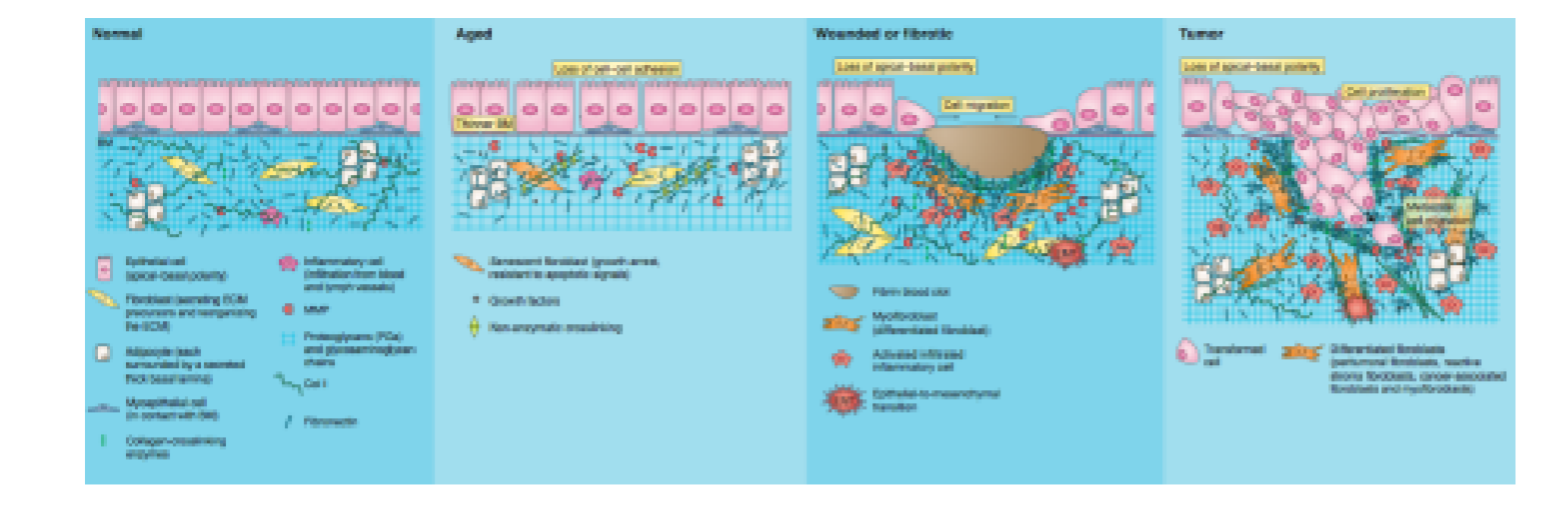
\includegraphics[width=1\textwidth]{ECMfunction.png}
\caption{\label{fig:ECM} ECM functionalization}
\end{figure}
\noindent
Figure \ref{fig:ECM}:the first example is a normal situation, good substrate. In an aged person we have a loss of elasticity. In the case of a wound, we observe a coagulation cascade and scar tissue formation - which is characterized by a compact tissue. The temporary material (crust) is used as scaffold. We can have healing by repair or regeneration. There is a higher rigidity in the case of temporary material. In the case of a tumour, we have an abnormal growth and migration inside - which they should not be present. The migration is caused by fibers not organising to close the hole.

\subsection{Surface chemistry: biorecognition in ECM}
Cell biology is governed by a complex series of interactions with the ECM. It is not enough to promote proliferation, we should control the adhesion involving the integrins (connected with few genes). We need a pool of molecules, since biological functions are orchestrated by a symphony of signals. Communication between cells and the cellular matrix is very relevant.
\\
\\
\noindent
A \textbf{biomaterial} is a substance that has been engineered to take a form which, alone or as a part of a complex system, is used to direct, by control of interactions with components of living systems, the course of any therapeutic or diagnostic procedure in human or veterinary medicine.
The aim is to recreate a basic environment before inducing regeneration. We need to upregulate proliferation at the beginning to create a population, then stop it for reaching ECM formation and achieving a therapeutic impact.
\noindent
Cells can interact with moving molecules through the gap junctions or through integrins; there are cells that must be very close e.g. skin, myocardium, in other cases integrins are mandatory. The ECM should also provide security for travelling molecules,  as molecules should not be degraded and must be kept in the active conformation.
Nutritional status is the bottle neck of tissue engineering, because in big wounds it is difficult to provide nutrition - as we need angiogenesis in order to have it. Hydrogels are cool because they can provide a lot of these requirements and can be combined to provide also mechanical support.
\\
\\
\noindent
The cell language is based on a mapping (micro- and nano-patterning) of biopolymers (dynamic ECM) shapes to their complementary binding. Chemical process during cell activity:
\begin{itemize}
\item Chemical reactions (irreversible): provide free energy (ATP $\rightarrow$ ADP)
\item Biopolymer (ECM) shape changes (reversible): provide control over chemical reactions
\end{itemize}

\subsection{Biocompatible materials: foundation ideas}
In order to design suitable materials, we should learn the biological pathways that lead to normal healing and reconstruction. Secondly, it is required to develop bio recognition surfaces that turn these pathways on and off. It is necessary to know specific affinities for the key molecules found in healing wounds that are associated with vascularised healing and regeneration (triggering local “unnatural” local healing).
If biomolecules are immobilised at the surface, they must be in the correct orientation and conformation. Porosity should be engineered to induce vascularisation and less fibrotic tissue. Furthermore, the modulus matching of scaffold-biomaterial should match with their intended use (modulus mismatch should exacerbate the FBRx).
Lastly, the engineered scaffold should be able to degrade into non-reactive substances at predetermined degradation rates to serve as a temporary guide for healing.

\section{Cell interactions}
Cells interact with the environment thanks to soluble factors, extracellular matrix and receptors.
Signals form ECM and neighbouring cells:
\begin{itemize}
\item gene expression regulation leads to adult stem cell differentiation [into the lineage of interest e.g. osteoblasts in bone]
\item tissue specific differentiation
\item survival of primary cells
\item Interaction with apoptosis: under external stimuli the cells may go to apoptosis. This may be useful in case of chemotherapy
\end{itemize}
The interaction between cells and matrix can be compared to a chemical reaction, where reagents can give rise to a reaction in a specific condition. Reactants are the cell + matrix, the specific condition is the biorecognition, we need integrins [without the plus (“+”) there is no reaction. All the reactants must communicate with each other. Integrins are important for response].
In order to achieve regeneration, we need to activate a number of functionalities, which should be listed according to time. The scaffold is a reactant, it is added in the bioreaction. Of course we also have mechanical stresses involved in the reaction. We need to take into account the control system, which should not be downregulated e.g. activate tissue regrowth and activate control system to stop when the tissue volume is enough.

\begin{figure}[h]
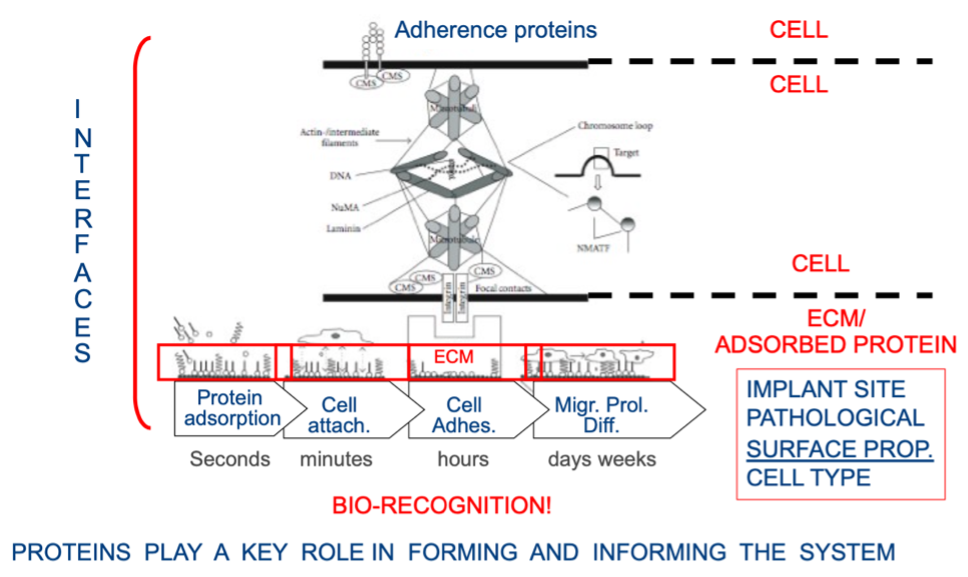
\includegraphics[width=1\textwidth]{interfaces}
\caption{\label{fig:interfaces}}
\end{figure}

\noindent
How does the body respond to the material?
Cells are in suspension in the culture, which contains serum (proteins). The surface first absorbs a coating of ions and proteins/lipids, which are then recognized and bound by cells.
Which kind of proteins will be absorbed by the implant? The quality of proteins depends on the chemical/mechanical properties of the scaffold and the context e.g. blood, skin, brain…For sure the first protein absorbed will be taken by plasma when we have bleeding. Depending on the proteins selected, the cells will adhere when the integrins of the cells can find some ligands among the proteins absorbed.
We only have cell adhesion when we have biorecognition of the scaffold.
\\
\\
\noindent
Surfaces must be designed in order to control protein absorption. Depending on the phenotype, we have different groups of integrins and also integrins specific for different genes.
The aim of TE is to promote cell adhesion through specific integrins needed to achieve regeneration. Scaffolds and cells are not isolated,  the empty spaces are filled by the ECM (providing proteins and water). This first step is crucial, depending on this we will reach failure or success. Therefore, the surface of the scaffold is really relevant. We can change the chemical properties, functionalize with new chemical groups, modify morphology to drive the interaction between scaffold and cells.
The interaction between the implant and biological systems is a dynamic process. The biomaterial is characterized by specific properties. If we incubate the material in a single protein solution, where the protein is in active conformation. Depending on the surface properties, the biomaterial will absorb the proteins, which will remain active, or we will witness deactivation / degradation / modification.
\begin{enumerate}
\item Protein is absorbed with original conformation = still active
\item Denaturation during absorption = not active, switch off
\item Different conformation = different activity [dangerous, unexpected situation]
\item Degradation = no specific activity, negative response and inflammation [small pro-inflammatory peptides are released into the environment]
\end{enumerate}
Having the protein active/inactive could be both positive or negative, it depends on what we need, what we want. The protein absorption mechanism is very dynamic, the absorbed proteins can also be released.
\\
\noindent
The protein substrate is important, we can change the material and see how it behaves.
We could observe different interactions with the proteins according to the starting material.Biocompatibility is a two-way process, the host affects the implant and vice versa. Also depending on the domain we will have a different adhesion, we can find differential adhesion distribution.
\\
\\
\noindent
\begin{figure}[h]
\centering
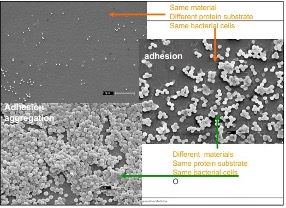
\includegraphics[width=0.5\textwidth]{polyu}
\caption{\label{fig:polyu}}
\end{figure}
\noindent
Figure \ref{fig:polyu}: the aim was to produce a surface avoiding bacterial infection. The polymer is polyurethane, used for catheter production - antibacterial properties are really required.
We see that the surface in contact with different protein substrates leads to different adhesion levels. When instead the protein substrate is equal with different materials, we see either adhesion or adhesion aggregation.
\\
\\
\noindent
\begin{figure}[h]
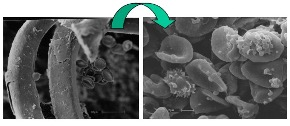
\includegraphics[width=0.5\textwidth]{vascular}
\centering
\caption{\label{fig:vascular}}
\end{figure}
\noindent
Figure \ref{fig:vascular}: vascular graft that failed after 6 years of implantation. The implant failed because the surface was completely destroyed. The bacterial cells (there was infection) adhered to the implant and this activated inflammatory response. Inflammatory cells digested the implant, made of a really strong polymer (same as parachutes). In addition, the implant started to detach in the circulation system + bacteria were able to attach to red blood cells. This is one of the few cases in which we do not want cell adhesion.

\subsection{Molecular mechanism of cell adhesion}
The orientation of ligands is critical for cell adhesion and biological function. The RGD sequence promotes cell adhesion and it is usually included in a long peptide – to avoid that RGD is involved in the link between cells, it would be invisible. Depending on the protocol parameters, we can achieve a nice or absent adhesion. The density is the same, the only difference is the orientation.
For instance we could have a different density of signal,  leading to a different outcome in adhesion. The density of signal is important for the function.  Our aim is to reach an equilibrium, not too much or too little adhesion. In the second scenario the cell is able to move, good choice if cells are required to migrate into the scaffold. If instead we need a fast formation of a layer we can choose the first case.
No absorption = no adhesion at all. This may be useful in some cases, e.g. in blood vessels to prevent thrombus, release of proteins from nanoparticles in cancer treatment.
Cell adhesion is mainly controlled by the surface. How can we know whether the conformation and orientation is correct? We can employ cell sensors, screening.

\begin{figure}[h]
\centering
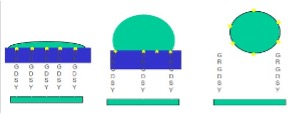
\includegraphics[width=0.5\textwidth]{adhesion}
\caption{\label{fig:adhesion}}
\end{figure}

\subsection{Cell adhesion}
Cell adhesion is a tightly regulated and dynamic biological process. It is central to physiological and pathological processes and critical to biomedical and biotechnological applications.
Adhesive interactions involve:
\begin{itemize}
\item anchorage (promotes migration, tissue organisation)
\item signaling (promotes activation, survival, proliferation, differentiation)
\end{itemize}

\begin{figure}[h]
\centering
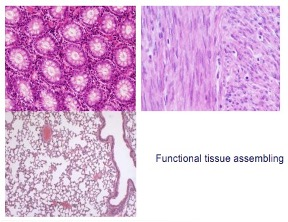
\includegraphics[width=0.5\textwidth]{functionaltissue}
\caption{\label{fig:funtis}}
\end{figure}
\noindent
In figure \ref{fig:funtis} starting from top left we see the functional tissue assembling of glands (radial section), muscles, and lung/alveolar tissue. In the case of muscles, functional tissue should support mechanical stress. In glands we have cells forming very well polarized tubes for transport, which are called capillary tubes. For lung tissue we have blood vessels, we need to have a small surface and permeability for gas exchange. The air should move into the bloodstream,  so the tissue should be very thin and adherent to the vessels. We have a low amount of ECM, the mechanical support is provided by cells themselves. The structure is function-dependent.
Assembly is driven by ECM and adhesion patterning. The morphology should depend on the function. Thin layer of ECM in the basal lamina, collagen fibrils. This provides elasticity, the fibrils are not a bundle, but organise somehow.


\subsection{Cell-material interactions}
Cells cannot adhere to synthetic surfaces, as there is no biorecognition (ECM performs better).
Cell adhesion to synthetic and bio surfaces occurs through a specific receptor interaction with adhesion protein/motifs:
\begin{itemize}
\item proteins adsorbed from physiological fluids (fibronectin, vitronectin, fibrogen)
\item ECM components present or deposited by cells (fibronectin, collagen, laminin)
\item biospecific sequences engineered on surfaces (RGC,YIGSR) for biorecognition
\end{itemize}
Adhesion receptor families are cadherins, selecting, HSPG, integrins, Ig superfamily.
Specific integrins act on specific receptors, so we must be precise. For instance, alpha5beta3 can recognize the ligands into fibronectin, collagen is recognized by alpha2beta1.
\\
\noindent
How to measure the adhesion strength of the cells? Experiment by Gallant and Garcia (2003). They provided two samples, performed centrifugation and measured cells attached and cells not adhered. In this way you can measure the difference in the strength of the adhesion.
\\
\\
\noindent
Depending on the surface chemistry, we will have a different cell adhesion rate.  According to the protein coating, e.g. either fibronectin or type I collagen, we will have different biological performance. A number of evaluation methods can give us an idea of the adherence strength.
\\
\\
\noindent
Figure \ref{fig:fibrin} design scaffold for neuron regeneration. Adhesion is necessary, but neurons also need to form connections with other neurons. RGD goal: neurite outgrowth, strategy: RGD- functionalization. They provided the material with fibrin, fibrin with low RGD and fibrin with high RGD. RGD is the classical adhesion peptide.
\begin{figure}[h]
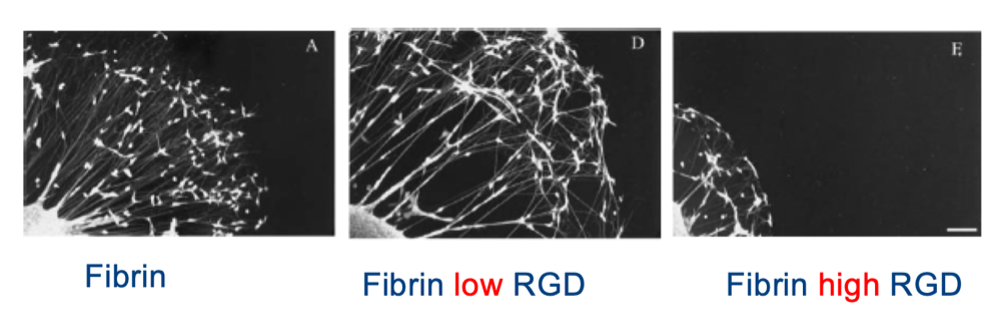
\includegraphics[width=1\textwidth]{fibrin}
\caption{\label{fig:fibrin}}
\end{figure}
\noindent
We observe a different response: high density is too much,  instead with a low amount of RGD we have a good outcome with a huge number of connections. When we increase RGD, the surface becomes more adhesive; this is mainly due to the fact that the cells are too sticky, but also because we must reproduce a biological environment. The amount of RGD should resemble the natural one. In fibronectin, the RGD content is 1 per chain, low amount. We have to move inside the natural range of pH, etc, … We want natural conditions. The language of the cells cannot be changed, we have to adapt our language. Signal is the combination of the ligand and density.
 \\
 \\
 \noindent
Adhesion is completely different in 2D and 3D. Cell adhesion is characterized by three stages: attachment cell body, flattening and spreading, and organization of the actin skeleton with the formation of focal adhesion between cell and its substrate. The strength of adhesion becomes stronger with the length of time a cell is allowed to adhere to a substrate or another cell.

\subsection{Cell organization}
The cell's adhesive interactions with the surrounding ECM (number of adhesive motifs, distribution, density) and neighbouring cells define cell shape and organisation, controlling functionality. This environment regulates the cell survival, differentiation, proliferation and migration.
\\
\\
\noindent
Chondrocytes are exposed to compressive forces, interstitial fluid flow and adhesive cues (cytokines) for cartilage maintenance. Chondrocytes are in a lacuna, they should behave like pillars and maintain their shape.
Soluble and matrix-bound GFs and flow induced mechanical forces on blood vessel wall, endos after polarity, cell-cell contacts, and degrade the surrounding basement membrane and stromal ECM in order to migrate and form tubular sprouts.
Adhesive and mechanical cues drive cell organization. Misregulation of the mechanism induces mechanical and structural changes in the ECM, and transformed epithelial cells migrate towards vasculature and eventually metastasize.
\\
\\
\noindent
ECM-dependent regulators can be associated with 2D, 1D and 3D migration. In turns influence intracellular pathways that govern the migratory phenotype. 3D are characterized by pore size and interconnection (cross linking degree). Aligned fibers are randomly distributed with low density in the scaffold.
\\
\\
\noindent
Adhesion and migration are controlled by the ECM composition, stiffness of the material and ligand density. While using fibers, something changes: by having a new parameter, aligned topography, we obtain different architectures. In the case of a mixed fibrous scaffold, we also have aligned/random, elastic behaviour, cross linking. Sending seed cells on the different structure, we will se diverse behaviour for orientation, migration, etc. Architecture can play a huge role.
\\
\\
\noindent
The substrate contractility regulates 3D migration, regardless of pore size. Stiff fibers vs soft fibers: when the cell lands on stiff fiber it can adhere, but becomes very stable and not able to modify the body/migrate. Instead cells on soft fibers are able to move and form protrusions.
Since cells in nature are connected to ECM fibers, when they move the ECM will also follow the contraction of the cell body. If the cell adheres to the soft fiber, the same natural movement can occur. When the substrate is too rigid contraction cannot occur, healing will be different. The scaffold should be soft enough to follow the reorganization needed by the cells.
\\
\\
\noindent
\begin{figure}[h]
\centering
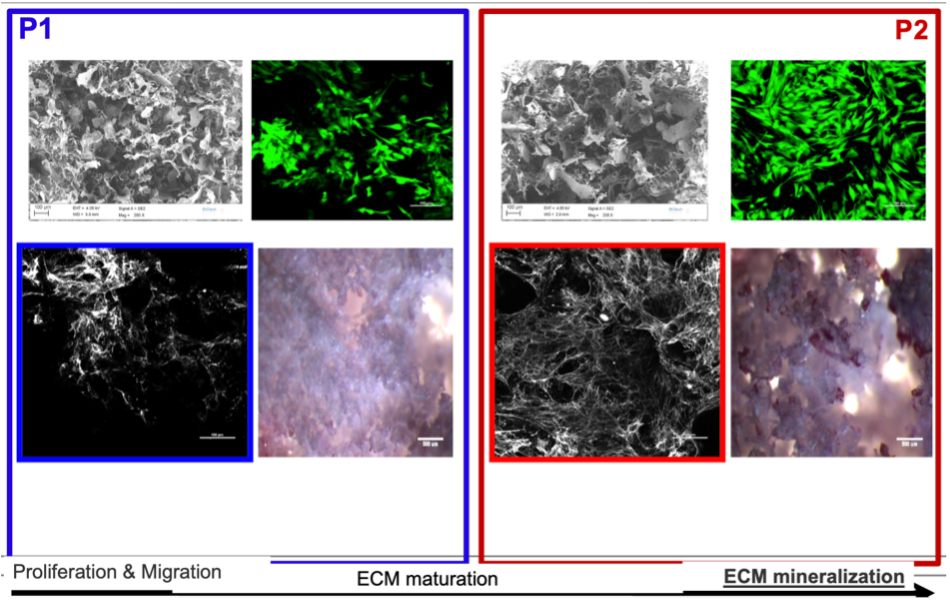
\includegraphics[width=0.7\textwidth]{mineralization}
\caption{\label{fig:min}}
\end{figure}
\noindent
Figure \ref{fig:min}: two scaffolds prepared with the same polymer, the difference is in pore size and distribution. The scaffolds are built for bone regeneration; we should take into account the presence of collagen fiber in a continuous network. Osteoblasts should infiltrate the scaffold for building the network, porosity should allow this. Once the network is formed, we have the deposition of the hydroxy apatite on top of collagen fibers.
Difference between P1 and P2 in terms of cell distribution: in P2 uniform, in P1 clusters (interconnection not complete). When we observe clusters of cells, we expect that the osteoblasts are not able to build a continuous network, due to tight collagen + no mineralization. When cells are not able to migrate, mineralization cannot occur.
A continuous network is also required for capillary formation. The parameters can be fully controlled with scaffold design. In order to improve the performance of P2 scaffold we could functionalize it with collagen or drug release systems.
\\
\\
\noindent
The scaffold surface interacts with the cell through the ECM (biorecognition). Our aim is to reproduce in vitro a working environment, working for the cell and solving a specific task. Depending on the context, we can have the bioreaction: the cell recognizes the surface of the scaffold if it is functionalized or for protein absorption. We have to refer to the cell population we are interested in, we have specific integrins.

\subsection{Methods for modulating receptor-ligand interactions}
\begin{enumerate}
\item Natural ECM biomaterials: biologically relevant environment, but poor mechanical properties and inconsistent reproducibility
\item Whole ECM adsorption
\item Synthetic linear binding motif: surface functionalization. We need to define the density of the signal, the protein of interest , the stability (quantify the time for which the signal should remain, orientation, homogeneous or pattern distribution.
\item Spatially oriented binding motif
\item Nanopatterning with nanolithography: mix different molecules and patterns, as well as technologies
\item ECM-like biomaterials
\end{enumerate}

\section{Biorecognition requirements}
The biorecognition process will have a good outcome only if the absorbed proteins are the right ones according to the following parameters:
\begin{itemize}
\item The absorbed proteins must contain sequences (ligands) recognizable by dedicated cellular receptors: among the first we remember RGD, YIGSR, IKVAV and RETTAWA, among the second we cite integrins. 
Integrins are heteromeric transmembrane receptors that mediate cell - ECM interaction with different glycoproteins (among whom fibronectin and vitronectin) and collagen fibers.
\item The ligands mentioned above must be oriented outward, they must not be hidden or used by the scaffold to link with the proteins. If this happens, the sequences won’t be able to be recognized by the cellular receptors.
\item The absorbed proteins must have a stable structure: they must not denature, take on conformations with unexpected functions (es: prions!) or hold native functions that could hinder the regenerative process (es: trigger clotting formation) or release peptides (that could be pro - inflammatory, leading to chronic inflammation).
\item The array of absorbed protein must expose the right number of ligands, with the right density.  In particular for the regenerative aim, we want our ligands to be in the right number and density to allow for macrophage adhesion while still allowing them to move. We also want them to stretch across the binding sites, since this stretching has been correlated with the polarization towards the M2 phenotype.
\end{itemize}




